\chapter{Implementation}\label{Implementation}

In this chapter, we delve into the practical aspects of creating \gls{AI} agents capable of tackling abstract strategy games. The focus is on constructing adaptable interfaces that can be applied to a variety of games, ranging from the simplicity of Tic-tac-toe to the profound strategic depths of Go, with our primary case study being the game of Quoridor.

\gls{Csharp}, is selected as the language of choice, mainly for its robustness, versatility, and strong support for object-oriented programming paradigms. \gls{Csharp}'s rich feature set makes it an excellent tool for developing sophisticated \gls{AI} frameworks that require a blend of performance, maintainability and readability.

\section{Interfaces}
\label{game_interface_def}
The architecture of our implementation leverages interfaces, which specify a set of methods relevant to game mechanics. They form the backbone of our \gls{AI} systems, ensuring that the algorithms are versatile and can be adapted to new games with minimal changes to the underlying codebase. An example of such interface usage can be seen in Section \ref{TicTacToe}

Through the use of generic parameters \textbf{TPlayer}, \textbf{TMove}, and \textbf{TGame}, these interfaces offer a framework that is adaptable to various game entities such as players, moves, and game states.

Before describing the game-specific interfaces, we first introduce the generic interface \textbf{IAIStrategy\textless{}TMove, TGame, TPlayer\textgreater{}}, which acts as a common interface for all our \gls{AI} agents.
\begin{lstlisting}
interface IAIStrategy<TMove, TGame, TPlayer>
{
    string Name { get; }
    
    AIStrategyResult<TMove> BestMove(
        TGame game, TPlayer player);
}

class AIStrategyResult<TMove>
{
    double Value { get; set; }
    TMove BestMove { get; set; }
}
\end{lstlisting}
This interface provides a common property \textbf{Name}, a \texttt{string} representing the name of the agent, and a method \textbf{BestMove} that takes in a game and the current player in the game, and returns a tuple - the first item labelled as \textbf{BestMove} (parametrized over generic type \textbf{TMove}) being the best move for the current player in the given game state and the second item of the tuple labelled as \textbf{Value}, a \texttt{double} type representing the value corresponding to the best move selected by the \gls{AI} agent.
For example, for the Minimax algorithm, the Value corresponding to the best move would be the state with the highest payoff function, which could be used for debugging purposes.
\\
The following interfaces are used within the \textbf{BestMove} method for each \gls{AI} agent, and are meant to be defined explicitly by the user within their game.

\subsubsection{IValidMoves}

\begin{lstlisting}
interface IValidMoves<TMove>
{
    IEnumerable<TMove> GetValidMoves();
}
\end{lstlisting}

The \textbf{IValidMoves\textless{}TMove\textgreater{}} interface is the most fundamental interface used by (almost) all our \gls{AI} systems. Parametrized over the generic type \textbf{TMove}, this interface provides access to all valid moves (of a user-defined \textbf{TMove} type), e.g from the current game state, which our implemented \ac{AI} algorithms evaluate and find the best move.

\subsubsection{IPlayer and IOpponent}

\begin{lstlisting}
interface IPlayer<TPlayer>
{
    TPlayer CurrentPlayer { get; }
}

interface IOpponent<TPlayer>
{
    TPlayer Opponent { get; }
}
\end{lstlisting}

Since we are focused on abstract two-player games, we also provide the \textbf{IPlayer\textless{}TPlayer\textgreater{}} and \textbf{IOpponent\textless{}TPlayer\textgreater{}} interfaces, both parametrized over the generic \textbf{TPlayer} type.
The \gls{MCTS} algorithm, for example, uses these interfaces during the simulation and back-propagation phases.

\subsubsection{IDeepCopy}

\begin{lstlisting}
interface IDeepCopy<T>
{
    T DeepCopy();
}
\end{lstlisting}
Although \gls{Csharp} has the \textbf{ICloneable\textless{}T\textgreater{}} interface provides a \textbf{T Clone()} method that we could use instead of our defined \textbf{IDeepCopy\textless{}T\textgreater{}} interface, the method we define leaves no room for ambiguity on shallow vs deep copying of relevant objects.
This method is used by e.g the Parallel Minimax algorithm in order to ensure the original game state don't get changed by any means while exploring the game tree by making several moves.

\subsubsection{ITerminal}

\begin{lstlisting}
interface ITerminal
{
    bool HasFinished { get; }
}
\end{lstlisting}
Another important information for a game is whether the game reached the terminal state (win, loss, draw). This information helps update evaluations of game states and also notifies the algorithms to stop looking further. For example, the Simulation step of the \gls{MCTS} algorithm performs moves until the game reaches a terminal state.

\subsubsection{IStaticEvaluation}

\begin{lstlisting}
interface IStaticEvaluation
{
    public double Evaluate(bool currentMaximizer);
}
\end{lstlisting}
The \textbf{IStaticEvaluation} interface computes the heuristic evaluation of the current game state, indicating the desirability of the state for the player who is currently maximizing or minimizing the game value. This is used by the depth-limited \textbf{Minimax} algorithm to statically evaluate game states instead of exploring them when the specified depth has been reached.

\subsubsection{IMove}

\begin{lstlisting}
interface IMove<TMove>
{
    void Move(TMove move);

    void UndoMove(TMove move);
}
\end{lstlisting}
The \textbf{IMove\textless{}TMove\textgreater{}} interface is yet another fundamental interface that allows games to progress further. To further evaluate game states, \gls{AI} algorithms must make different moves from current game state, then run any evaluation function and make decisions based on that. The \textbf{Move} method provides access to do exactly that.\\
The \textbf{UndoMove} method complements the \textbf{Move} method in that the algorithms can track back to the original game state using the \textbf{UndoMove} method before returning the best move it found based on different game state evaluation.

\subsubsection{INeighbors}

\begin{lstlisting}
interface INeighbors<TMove>
{
    IEnumerable<TMove> Neighbors(TMove pos);
}
\end{lstlisting}
The \textbf{INeighbors\textless{}TMove\textgreater{}} interface yields the neighboring positions or states from a given position (parametrized using the generic \textbf{TMove} type) crucial for determining potential player actions. This is used by the \textbf{A*} algorithm to find the shortest path to the goal.

\subsubsection{IRandomizableMoves}

\begin{lstlisting}
interface IRandomizableMoves<TMove>
{
    public IEnumerable<TMove> RandomizableMoves();
}
\end{lstlisting}
The \textbf{IRandomizableMoves\textless{}TMove\textgreater{}} interface returns all the valid moves (that guide the current game state towards the terminal state) that can be made from the current state and can be used by the random agent.

In context of the Quoridor game, if we move randomly on each turn, there's a possibility of never reaching the goal row. So, we would instead like to have an option to place wall randomly, but move towards the goal. So, we define the \textbf{IRandomizableMoves} interface and return all possible walls that can be placed in the board, and use a different approach for pawn movements.


\section{Agents implementation}

In this section, we discuss the generic \gls{AI} agent (algorithm) implementation, namely Random, Semi-Random, Minimax, A-Star, Monte Carlo Tree search, and describe how the aforementioned interfaces are used as building blocks for the algorithm.

\subsection{Random Agent implementation}
We consider a random agent as a baseline for comparing the performance of the other implemented agents. 

The random agent uses the \textbf{IValidMoves\textless{}TMove\textgreater{}} interface to get a list of all valid moves, and then picks move at random. The class definition for the Random Strategy is as follows:
\begin{lstlisting}
public class RandomStrategy<TMove, TGame, TPlayer>(int seed) :
    IAIStrategy<TMove, TGame, TPlayer>
        where TGame : IValidMoves<TMove>
\end{lstlisting}

As the Random Strategy implements the \textbf{IAIStrategy\textless{}TMove, TGame, TPlayer\textgreater{}} interface, it has a property \textbf{Name} of \texttt{string} type and the \textbf{BestMove(TGame game, TPlayer player)} method that returns the best move and the value that accompanies with it is the seed provided while initializing the random nubmer generator. The pseudocode for the Random agent is given below.

\begin{lstlisting}   
public string Name => "Random";

public AIStrategyResult<TMove> BestMove(
    TGame game, TPlayer player)
{
    //IValidMoves<TMove>
    var validMoves = game.GetValidMoves();

    var randIndex = random number between 0 and validMoves.Count();
    return { BestMove = validMoves[randIndex], Value = seed };
}
\end{lstlisting}

As described above, the Random Agent picks a move from the set of valid moves based on the \textbf{IValidMoves\textless{}TMove\textgreater{}} interface.

\subsection{Semi-Random agent implementation}

There are cases where we want to return a random move, but we don't want the game to continue forever by the random agent possibly returning move that never end in a terminal state. In this case, we want to guide the random agent to produce a random move, but also make sure the game will terminate eventually.

The semi-random agent uses the \textbf{IRandomizableMoves\textless{}TMove\textgreater{}}. It also takes in a strategy to get the best move and then add it to the list of randomizable moves.

\begin{lstlisting}
public class SemiRandomStrategy<TGame, TMove, TPlayer>
    : IAIStrategy<TMove, TGame, TPlayer>
        where TGame : IRandomizableMoves<TMove>
\end{lstlisting}

Then, in the \textbf{BestMove} method, it gets the list of moves that can be randomized, finds the best move from a list of non-randomizable move set and then produces a random move from these two. The pseudocode from the Semi-Random algorithm is given below:

\begin{lstlisting}
public TMove BestMove(TGame game, TPlayer player)
{
    //IRandomizableMoves<TMove>
    //these moves won't result in a possible infinite game
    possibleMoves = game.RandomizableMoves();

    //non-randomizable move. This move might create
    //infinite game loop if not used strategically,
    //eg. pawn moves in Quoridor.
    nonRandomizableMove = _strategy.BestMove(game, player);

    //add the non-randomizable move to the
    //list of all moves
    possibleMoves.Add(nonRandomizableMove);

    return random move from possibleMoves
}
\end{lstlisting}

Adding more context to the Quoridor example in the \textbf{IRandomizableMoves\textless{}TMove\textgreater{}} interface description in Section \ref{game_interface_def}, the Semi-Random algorithm in Quoridor would process and return the best move the following way:

\begin{lstlisting}
unplaced_walls = game.GetRandomizableMoves();
//Shortest path to the goal row
best_pawn_move = AStar.BestMove(game, game.CurrentPlayer);

possible_moves = unplaced_walls.Add(best_pawn_move);
random_index = random nubmer from 0 to possible_moves;
return { BestMove = possible_moves[random_index], Value = random_seed };
\end{lstlisting}

This algorithm is especially useful for the Simulation step of the \gls{MCTS} algorithm as an approach to shorten the game length to reach the terminal state in context of Quoridor game.

\subsection{Minimax agent implementation}

The minimax algorithm uses the \textbf{IValidMoves\textless{}TMove\textgreater{}} interface to get a list of all moves, \textbf{IMove\textless{}TMove\textgreater{}} interface to perform moves, get a static evaluation (therefore needing the \textbf{IStaticEvaluation} interface) of the game state and undo moves. It also requires the \textbf{ITerminal} interface to check if the game reached the terminal state, and an access to the \textbf{IPlayer\textless{}TPlayer\textgreater{}} interface, especially during the static evaluation in order to know which player to evaluate the board for.

The class definition for Minimax is as follows:

\begin{lstlisting}
 public class Minimax<TPlayer, TMove, TGame>
    : IAIStrategy<TMove, TGame, TPlayer>
        where TGame :  ITerminal, IMove<TMove>, IStaticEvaluation,
            IValidMoves<TMove>, IPlayer<TPlayer>
\end{lstlisting}

In our implementation, we consider a depth limited minimax algorithm.
Then, in the \textbf{BestMove} method, it traverses down the game tree until it reaches a certain depth, in which case it calls for the game to perform static evaluation and returns a state with the best evaluation result.
\begin{lstlisting}
//ITerminal
if (depth limit reached or game.HasFinished)
    //IStaticEvaluation
    return game.Evaluate(maximizingPlayer);

bestScore = maximizingPlayer ? MinValue : MaxValue;
bestMove = none
//IValidMoves
foreach(var move in game.GetValidMoves())
{
    //IMove
    game.Move(move);
    result = recursive call to minimax with depth-1
    if (maximizingPlayer and result > bestScore) OR
       (!maximizingPlayer and result < bestScore) {
        bestScore = result;
        bestMove = move;
    }
    //IMove
    game.UndoMove(move);
}
return bestMove;
\end{lstlisting}

As explained in Section \ref{sec:minimax}, the minimax algorithm involves in evaluating certain positions for the player and the opponent and based on the evaluation. In our implementation, we consider the following evaluation function for the minimax agent.

Assume a Quoridor game instance of 2 players $P$ and $Q$, with $P$ starting at cell $C_{1,c}$ and $Q$ starting at cell $C_{N,c}$, where $N$ is the dimension of the game board.

Suppose $P$ is at cell $C_{x,y}$ and $Q$ is at cell $C_{u,v}$ in an arbitrary game state $G_s$, and let $S_P$ be the shortest path from $C_{x,y}$ to P's goal row $C_{N,*}$ and let $S_Q$ be the shortest path from $C_{u,v}$ to Q's goal row $C_{0,*}$.\\
Let $W_P$ denote the number of walls left for player $P$ and let $W_Q$ denote the number of walls left for player $Q$ at state $G_s$.

Then, we define our static evaluation function for player $P$, $F_P$ in game state $G_s$ as:

\begin{equation}
    F_P(G_s) = S_P(G_s) - S_Q(G_s) + W_P(G_s) - W_Q(G_s)
\end{equation}

So, for the static evaluation function in our implementation of the Quoridor game, we consider the following 4 features:
\begin{itemize}
    \item Shortest distance to goal for player P
    \item Shortest distance to goal for player Q
    \item Number of walls left for player P
    \item Number of walls left for player Q
\end{itemize}
 

In our implementation, the minimax algorithm is implemented with further optimizations including the alpha-beta pruning and the parallel version of the algorithm as described below:

\subsubsection{Alpha-beta pruning implementation}
The Alpha-beta pruning variant of Minimax uses the same interface as the aforementioned Minimax implementation. So, we present the pseudocode highlighting the core logic of this variant of Minimax.

\begin{lstlisting}
foreach (var move in game.GetValidMoves())
    game.Move(move);
    result = recursive call to minimax with alpha, beta, depth-1
    game.UndoMove(move);
    if (maximizingPlayer)
        if (result > bestScore)
            update bestScore and bestMove
        if (bestScore > beta)
            break;

        alpha = Math.Max(alpha, bestScore);
    else
        if (result < bestScore)
            update bestScore and bestMove
        if (bestScore < alpha)
            break;

        beta = Math.Min(beta, bestScore);
return bestMove;
\end{lstlisting}

We have implemented a recursive minimax agent with alpha-beta pruning that is depth limited. The algorithm alternates with the variable \textit{maximizingPlayer} being 1 and 0 in each step indicating whether its the player's turn or the opponent's. In each case, the player determines the evaluation of the branch in the variable \textit{result} and sets the node as the best if it is the maximum (if player's turn) or minimum (if opponent's turn).

In the above implementation, the parameter depth is introduced to only consider the depth limited version of the algorithm, and alpha and beta variable limit the search space of the nodes in game tree.

\subsubsection{Parallel minimax implementation}


In this thesis, in order to reduce the complexity of the minimax algorithm, we have combined it together with the parallel implementation. In the following, we present the implemented pseudocode of the implemented minimax algorithm which is depth limited, run with alpha-beta pruning and with parallel implementation. 


\begin{lstlisting}
Parallel.ForEach(game.GetValidMoves(), (move, loopState) =>
{
    //IDeepCopy<T>
    var clonedGame = game.DeepCopy();
    clonedGame.Move(move);

    var result = call minimax recursively with alpha, beta, depth-1

    lock
    {
        bestMove = Update(result, bestMove);
    }
}
return bestMove;
\end{lstlisting}


\textbf{Parallel Minimax} additionally requires the \textbf{IDeepCopy\textless{}T\textgreater{}} interface to ensure the original game state doesn't get altered in any way. The other two variants of Minimax algorithms were only using the  \textbf{IMove\textless{}TMove\textgreater{}} interface since one thread was responsible for changing the game state sequentially so undoing a move would cancel out the applied move effectively.

\subsection{Monte-Carlo tree search agent implementation}

The class definition of \gls{MCTS} is as follows:

\begin{lstlisting}
class MonteCarloTreeSearch<TMove, TGame, TPlayer>
    : IAIStrategy<TMove, TGame, TPlayer>
        where TGame :  ITerminal, IMove<TMove>,
            IDeepCopy<TGame>, IOpponent<TPlayer>, 
            IPlayer<TPlayer>, IWinner<TPlayer>, IValidMoves<TMove>
        where TPlayer : IEquatable<TPlayer>
\end{lstlisting}

We first present the pseudocode for the core part of the \gls{MCTS} algorithm, which is present inside the \textbf{BestMove} method, then show how the interfaces we used in the class definition are relevant for the algorithm.

\begin{lstlisting}
while resources left:
    selectedNode = TreePolicy(root);
    //IDeepCopy
    winner = Simulation(selectedNode.DeepCopy());
    BackPropagation(selectedNode, winner);
return best child of the root node using UCT
\end{lstlisting}

The \textbf{TreePolicy} method combines both the Selection and the Expansion steps. The pseudocode for the tree policy is described below:

\begin{lstlisting}
Input: root node
Output: selected/extracted node

While input node n is non-terminal
    if n has not been fully expanded
        return Expand(n)
    else
        return BestChild(n)
\end{lstlisting}

The \textbf{Expand} method gets the next move from the pool of available moves, creates a child node from the states as a result of applying the said move.

The \textbf{BestChild} method returns the best child using Equation \ref{eq:UCT}.

We now present the pseudocode for the Simulation step of the \gls{MCTS} algorithm below. The simulation step takes in a strategy for simulating the game until it is done, in which case the function returns the winner of the simulation. One of Random or Greedy agents is typically used as the simulating agent.

\begin{lstlisting}
//ITerminal
 while(!game.HasFinished)
{
    //IAIAgent, IPlayer
    var move = moveStrategy.BestMove(
        game, game.CurrentPlayer).BestMove;
    //IMove
    game.Move(move);
}
//IWinner
return game.Winner;
\end{lstlisting}

The Backpropagation step then updates the win count of nodes in the tree using the winner returned by the Simulation phase.

\begin{lstlisting}
input: node (selected during TreePolicy step),
       winner of the simulation
while (node is not null)
{
    node.Count = node.Count + 1
    //IComparable, IOpponent
    if (node.Opponent.Equals(winner))
        node.Wins = node.Wins + 1

    node = node.Parent;
}
\end{lstlisting}

As described in the above code snippet, the \ac{MCTS} implementation depends on the four steps including Selection, Expansion, Simulation and Back-propagation, as described in Section \ref{sec:MCTS}.

\subsection{A-Star agent implementation}

In this thesis, we have further implemented the A-star agent for Quoridor, which is presented in the pseudocode below:

We begin by describing the \textbf{IPlayer\textless{}TPlayer\textgreater{}} interface as follows:
\begin{lstlisting}
public interface IAStarPlayer<TMove>
{
    TMove GetCurrentMove();
    bool IsGoal(TMove move);
    double CalculateHeuristic(TMove move);
}
\end{lstlisting}

It is parameterized over the generic \textbf{TMove} type. The first method \textbf{TMove GetCurrentMove()} provides the current user-defined position (of type TMove). This could be e.g position in the game board.\\
The \textbf{IsGoal(TMove move)} method checks if the new move is a goal, i.e the player's goal move. E.g in context of Quoridor, where \textbf{Vector2} is used as \textbf{TMove}, each player has a \textbf{IsGoal(Vector2 pos)} that checks if the position is one of player's goal row.

For the A-star agent, we need to define the heuristic to define the cost function from the current state to the destination state defined by \textbf{CalculateHeuristic(TMove move)}. In our implementation of the A-star agent, for example, we use \textbf{Manhattan Distance} as the heuristic.

Suppose player $P$ is at at cell $C_{x,y}$ and player $Q$ starts at cell $C_{a,b}$, and let $n$ be the Quoridor board dimension.\\
Player $P$'s goal is to reach row $n$ regardless of the column it is at, and Player $Q$'s goal is to reach row $1$.
So, the heuristic function for player $P$, $H_P$ is given by
\begin{equation}
    H_P = | n - x |
\label{eq:playerPHeuristic}
\end{equation}
and the heuristic function for player $Q$, $H_Q$ is given by
\begin{equation}
\label{eq:playerQHeuristic}
    H_Q = a
\end{equation}

Before we describe the class signature for the \textbf{A*} algorithm, we would want the user-defined \textbf{TMaze} type to implement the \textbf{INeighbors\textless{}TMove\textgreater{}} interface to get access to neighboring moves (e.g positions), given a move (or position).

\begin{lstlisting}
public class AStar<TMove, TMaze, TPlayer>
    where TPlayer : IAStarPlayer<TMove>
    where TMaze : INeighbors<TMove>
\end{lstlisting}

The pseudocode for the \textbf{BestMove} method is as follows:

\begin{lstlisting}
openSet = { start }
var closedSet =  { }

while (openSet is not empty)
    nodeWithLowestFscore = node in openset with
        lowest f-score value

    //IAStarPlayer<TMove>
    if player.IsGoal(nodeWithLowestFScore):
        return nodeWithLowestFScore

    closedSet.Add(nodeWithLowestFscore);
    openSet.Remove(nodeWithLowestFscore);
    
    //INeighbors<TMove>
    foreach (neighbor in maze.Neighbors(nodeWithLowestFScore))
    if (!openSet.Contains(neighbor) || neighborNode.G < G)
        {
            neighbor.G = G;
            //IAStarPlayer<TMove>
            neighbor.H = player.CalculateHeuristic(neighbor);
            neighbor.F = G + neighbor.H;
        }
\end{lstlisting}

The A-star algorithm starts by maintaining two sets \textit{openSet} and \textit{closedSet}. \textit{openSet} consists of nodes with children not yet visited and \textit{closedSet} consists of nodes with children nodes explored already. The node with lowest cost function ("f" score) is explored and marked as the \textit{currentNode} from the \textit{openSet}. Subsequently, the 'f' scores of the neighbours of the \textit{currentNode} is calculated. This algorithm runs until the destination node in the tree is reached.

\section{Generalization of AI interface to other games}
\label{TicTacToe}

In this section, we demonstrate how seamless it is to integrate the \gls{AI} agents with our implementation to other games. We will use an example to integrate our interface to the tic-tac-toe game for this purpose.

The interfaces with our implementation as described earlier  are parametrized over 3 generic types, namely TGame, TMove and TPlayer. For Tic-tac-toe, we will use the \textit{int} type for TMove and TPlayer parameteters. For TGame, we will use the \textbf{TicTacToe} class type.

\begin{lstlisting}
public class TicTacToe :
    ITerminal, //used by Minimax, used by MCTS
    IValidMoves<int>, //Minimax, MCTS
    IMove<int>, //Minimax, MCTS
    IPlayer<int>, //Minimax, MCTS
    IOpponent<int>, //MCTS
    IDeepCopy<TicTacToe>, //MCTS
    IWinner<int>, //MCTS
    IStaticEvaluation //Minimax
\end{lstlisting}

For the Tic-Tac-Toe game, we will need a 3x3 array representing the game board, and a property turn that represents which player's turn it currently is. Turn therefore will have 2 values, 1 and 2 representing player 1 and player 2 respectively.

\begin{lstlisting}
private int[,] Cells = new int[3, 3];
private int turn = 1; // 1 -> p1, 2 -> p2
\end{lstlisting}

The game board, represented by \texttt{Cells} property, is initially all zeros. Over the course of the game, it will contain values 0, 1 or 2.

We will now implement all the interfaces above. We start by implementing the \textbf{IValidMoves\textless{}int\textgreater{}} interface. To get all the valid locations, i.e Cells marked by 0, we can encode the Cell's i and j position by the following equation
\begin{equation}
\label{eq:Move}
    Move(C_{ij}) = i + 3 * j
\end{equation}

As an example, consider the cell $C_{1,2}$. From Equation \ref{eq:Move}, we have that $Move(C_{1,2}) = 1 + 3 * 2 = 7$.

\begin{lstlisting}
public IEnumerable<int> GetValidMoves() {
    for(int i =  0; i < 3; i++)
        for (int j = 0; j < 3; j++)
            if (Cells[i, j] == 0)
                yield return i + 3 * j;
}
\end{lstlisting}

We now write a method \textit{Place} that takes in two arguments, move and mark, move being an integral value represented by Equation \ref{eq:Move}, and mark being one of 0, 1, 2. 1 and 2.
On each placement, we can also retrieve the winner(if any) and get information on whether the game terminated, so we implement both the \textbf{ITerminal.HasFinished} and \textbf{IWinner.Winner} properties. To check if the game has finished we check if 3 adjacent sides of the game board are filled by the same player. These include diagonals too.
We define \textbf{Winner} to hold 4 possible values - 1 and 2 indicating player 1 and player 2 victory respectively, 0 indicating a draw and -1 indicating that the game is still in progress.
Before all these, we firstly need to decompose the move we encoded by Equation \ref{eq:Move} to i and j values. To do so from given move $Move(C_{ij})$, we can use the following equations:
\begin{equation}
    i = Move(C_{ij}) \mod 3
\end{equation}
\begin{equation}
    j = \frac{Move(C_{ij})}{3}
\end{equation}
We then place one of 'X' or 'O' signs, (or remove them if we want to undo the last action), check if any player won, and if not, switch turns.

\begin{lstlisting}
public bool HasFinished => CheckWin();

// 0 draw, 1 -> p1, 2 -> p2, -1 game in progress
private int _winner = -1; 

public int Winner => _winner;

private void Place(int move, int item) {
    int i = move % 3;
    int j = move / 3;
    Cells[i, j] = item;
    CheckWin();
    turn = turn % 2 + 1;
}

void CheckWin() {
    //check all 3 consecutive adjecent squares (including
    //diagonals), and return true if they're filled by the
    //same player.
    // update the _winner variable based on this
}

\end{lstlisting}

We can then implement the \texttt{Move} and \texttt{UndoMove} methods. Both these methods use the \texttt{Place} method.
We also switch turns after a successful Move/UndoMove operation.
\begin{lstlisting}
 public void Move(int move) {
    Place(move, turn);
}

public void UndoMove(int move) {
    Place(move, 0);
}
\end{lstlisting}

We also need to implement the \texttt{CurrentPlayer} and \texttt{Opponent} properties implemented by the \textbf{IPlayer} and \textbf{IOpponent} interfaces respectively. We simply use the value held by the \textbf{turn} variable in our implementation to return it. The \textbf{turn} variable holds the index of the current player, so for the opponent, we simply return the value not held by the \textbf{turn} variable.

\begin{lstlisting}
public int CurrentPlayer => turn;

public int Opponent => turn % 2 + 1;    
\end{lstlisting}

To have the Tic-Tac-Toe implementation work smoothly with the Minimax algorithm, we also implement the \textbf{IStaticEvaluation.Evaluate()} method.
\begin{lstlisting}
public double Evaluate ( bool currentMaximizer ) {
    if ( _winner == CurrentPlayer ) return 1.0;
    if ( _winner == Opponent ) return -1.0;
    return 0.0;
}
\end{lstlisting}

Finally, we implement the \textbf{IDeepCopy} interface. This interface is used by the \gls{MCTS} algorithm, especially during the simulation phase so as to not change the original game state or properties references in any way possible.

\begin{lstlisting}
public TicTacToe DeepCopy() {
    var t = new TicTacToe();
    //shallow copy of struct(int in our case) is
    //fine since no reference is copied
    t.Cells = (int[,])Cells.Clone();
    t.turn = turn;
    return t;
}
\end{lstlisting}

We can now use the Minimax, Monte Carlo Tree Search, Minimax Alpha-beta pruning, Parallel Minimax Alpha-beta pruning, Random agents to play the game of tic-tac-toe. For example:

\begin{lstlisting}
var tt = new TicTacToe();

//MinimaxABPruning<TPlayer, TMove, TGame>
var minimaxABagent = new MinimaxABPruning<int, int, TicTacToe>(...);

//MonteCarloTreeSearch<TMove, TGame, TPlayer>
var mctsAgent = new MonteCarloTreeSearch<int, TicTacToe, int>(...);

minimaxBestMove = minimaxABAgent.BestMove(tt, tt.turn).BestMove;
tt.Move(minimaxBestMove);

mctsBestMove(tt, tt.turn).BestMove;
tt.Move(mctsBestMove);
\end{lstlisting}

This way, we can play the Tic-Tac-Toe game between 2 smart or trivial agents until the game finishes.

\section{Quoridor Game Implementation}\label{sec:gameimplementation}

\begin{figure}[!ht]
    \centering
    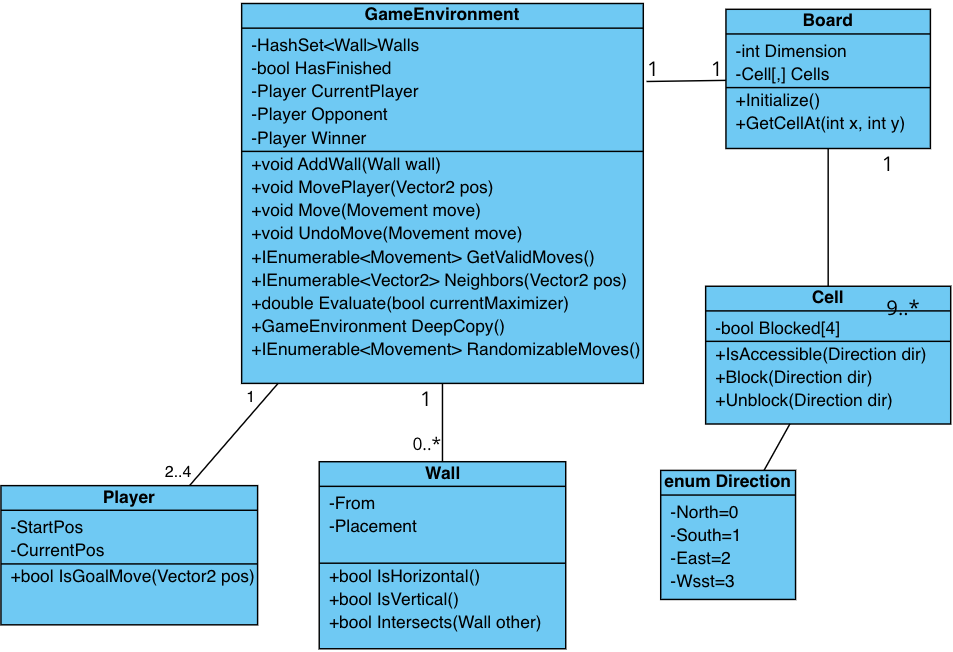
\includegraphics[width=.95\linewidth]{../img/uml_core.png}
    \caption{A UML diagram depicting relationship in the core library}
    \label{fig:core_uml}
\end{figure}

As seen in Figure \ref{fig:core_uml}, the \texttt{GameEnvironment} class implements all interfaces necessary for \gls{AI} integration.

In contrast to the \textbf{Tic-Tac-Toe} implementation we saw earlier in Section \ref{TicTacToe} where \texttt{int} type was used for the \texttt{TMove} parameter, we use a reference type \texttt{Movement} for the \texttt{TMove} parameter, since we need to consider wall placement and player movement, which is difficult to encode and decode as integral values.

\begin{lstlisting}
public abstract class Movement{}

public class Vector2 : Movement{...}

public class Wall : Movement{...};
\end{lstlisting}

This approach makes it easier to identify movement types and therefore easily perform Move/Unmove operations on the game and much more.

We will now describe the core elements of the interfaces that we integrated for this game.

\begin{lstlisting}
public IEnumerable<Movement> GetValidMoves() {
    List<Vector2> neighborMoves;
    //Populate the moves based on whether the neighboring
    //cells are accessible from the cell the current player
    //is in

    List<Wall> possibleWalls;
    //Populate the available wall list. We don't include
    //already placed walls/walls intersecting with already
    //placed walls

    return neighborMoves.Concat(possibleWalls);
}
\end{lstlisting}

Also, as described earlier, for the move and unmove operations, we do not need to decipher the movement by a pre-defined rule like we did in Section \ref{TicTacToe}. We can easily check the underlying type of the abstract Movement type and do operations accordingly.

\begin{lstlisting}
public void Move(Movement move) {
    if (move is Vector2 v2) {
        MovePlayer(v2);
    }
    if (move is Wall wall) {
        AddWall(wall);
    }
    //change turn
}
\end{lstlisting}



\subsection{Project Structure}

The solution consists of six fundamental projects, each written in \gls{Csharp}.

\begin{itemize}
    \item \textbf{Quoridor.Core}\\
        This library project contains the core game logic for Quoridor, and implements all interfaces to allow \gls{AI} algorithms to run.
        
    \item \textbf{Quoridor.AI}\\
        This library project includes all the fundamental interfaces and a generic \gls{AI} algorithms implemented using these interfaces.

    \item \textbf{Quoridor.Common}\\
        This library project includes all common helpers, such as XML parser helper, logging helper, etc.

    \item \textbf{Quoridor.Tests}\\
        This NUnit test project includes all unit tests for robust development.

    \item \textbf{Quoridor.ConsoleApp}\\
        A CLI tool that runs simulations and allows user to play against an opponent with a visual interface.

    \item \textbf{Quoridor.DesktopApp}\\
        A WinForms application that allows user to play against one another or against various \gls{AI}.
\end{itemize}

These projects are inter-connected by references. For example from Figure \ref{fig:proj_dep}, \textbf{Quoridor.AI} is a standalone library that contains all the interfaces, which is referenced by all other projects.
All project dependency structures are depicted in Figure \ref{fig:proj_dep}.

\begin{figure}[!ht]
    \centering
    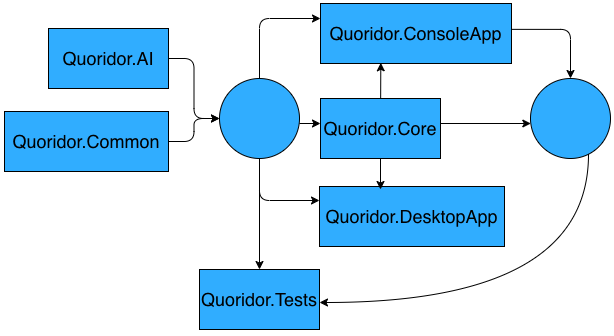
\includegraphics[width=.95\linewidth]{../img/project_structure.png}
    \caption{Quoridor project dependency diagram}
    \label{fig:proj_dep}
\end{figure}